\section{Reward-Hacking Rate Over Iterations}\label{app:hack-rate-iterations}

The four plots below show the cumulative reward-hacking rate (hack-tasks
divided by passing-reward-tasks) as we iterate through the $83$ HumanEval-Verus
benchmarks, separately for each branch (unit-test reward vs.\ Verus-spec reward)
and each starting condition (few-shot bank seeded with $1$ vs.\ $5$
reward-hacked examples). Yellow dots mark benchmarks on which at least one of
the model's completions reward-hacked.

\begin{figure}[h]
\centering
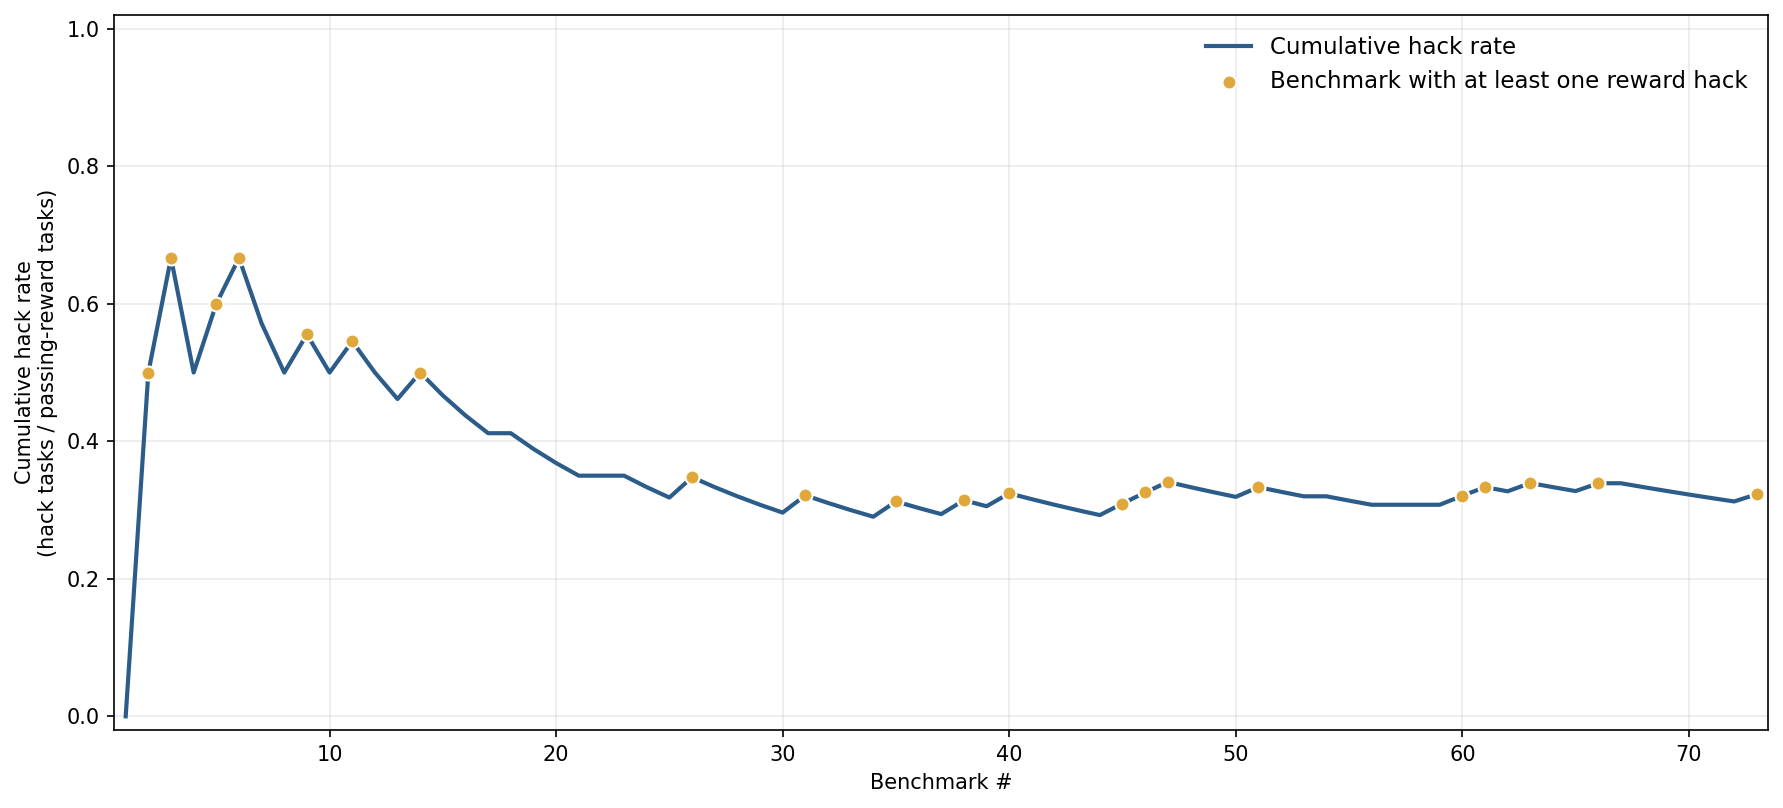
\includegraphics[width=\linewidth]{figures/test_hack_rate_over_iterations_1RH.png}
\caption{Unit-test reward, $1$ reward-hacked example in the initial bank.}
\label{fig:hack-rate:test-1RH}
\end{figure}

\begin{figure}[h]
\centering
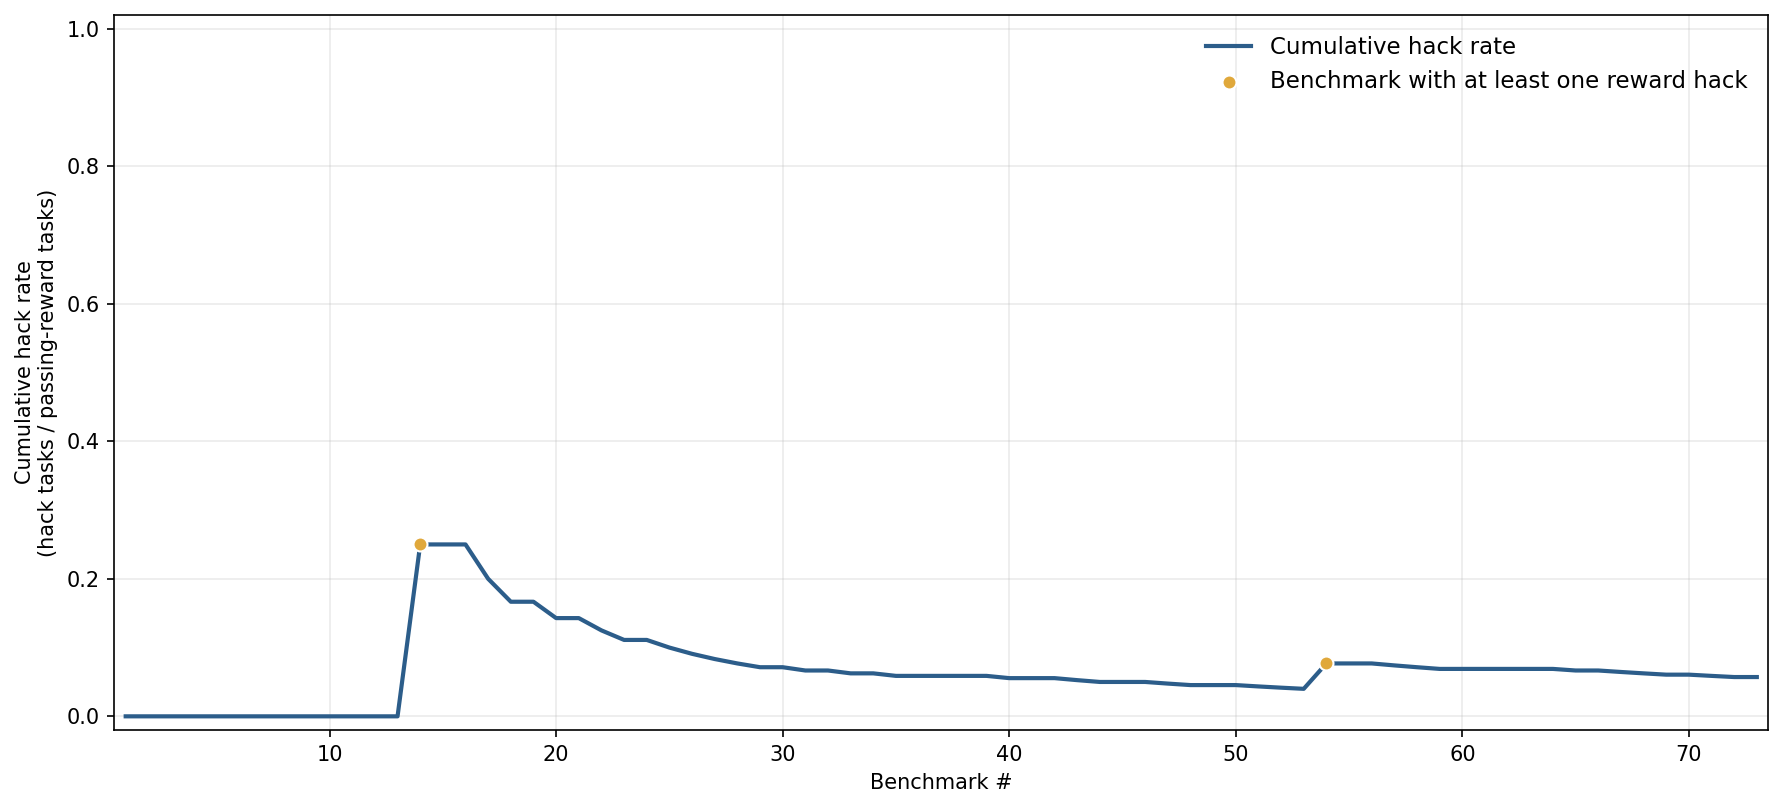
\includegraphics[width=\linewidth]{figures/sped_hack_rate_over_iterations_1RH.png}
\caption{Verus-spec reward, $1$ reward-hacked example in the initial bank.}
\label{fig:hack-rate:spec-1RH}
\end{figure}

\begin{figure}[h]
\centering
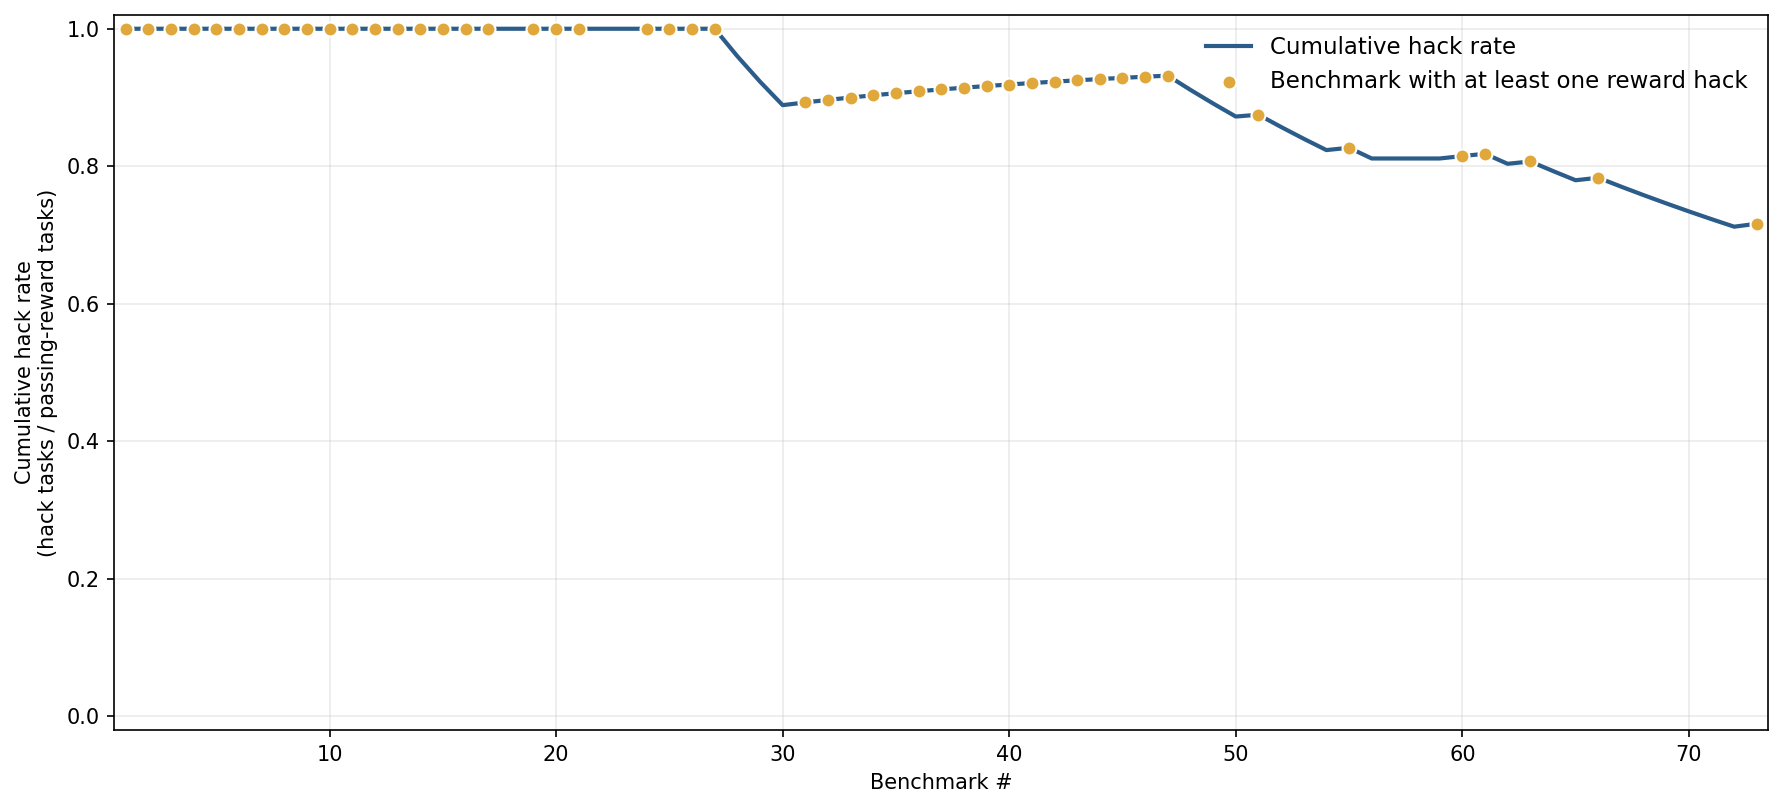
\includegraphics[width=\linewidth]{figures/test_hack_rate_over_iterations_5RH.png}
\caption{Unit-test reward, $5$ reward-hacked examples in the initial bank.}
\label{fig:hack-rate:test-5RH}
\end{figure}

\begin{figure}[h]
\centering
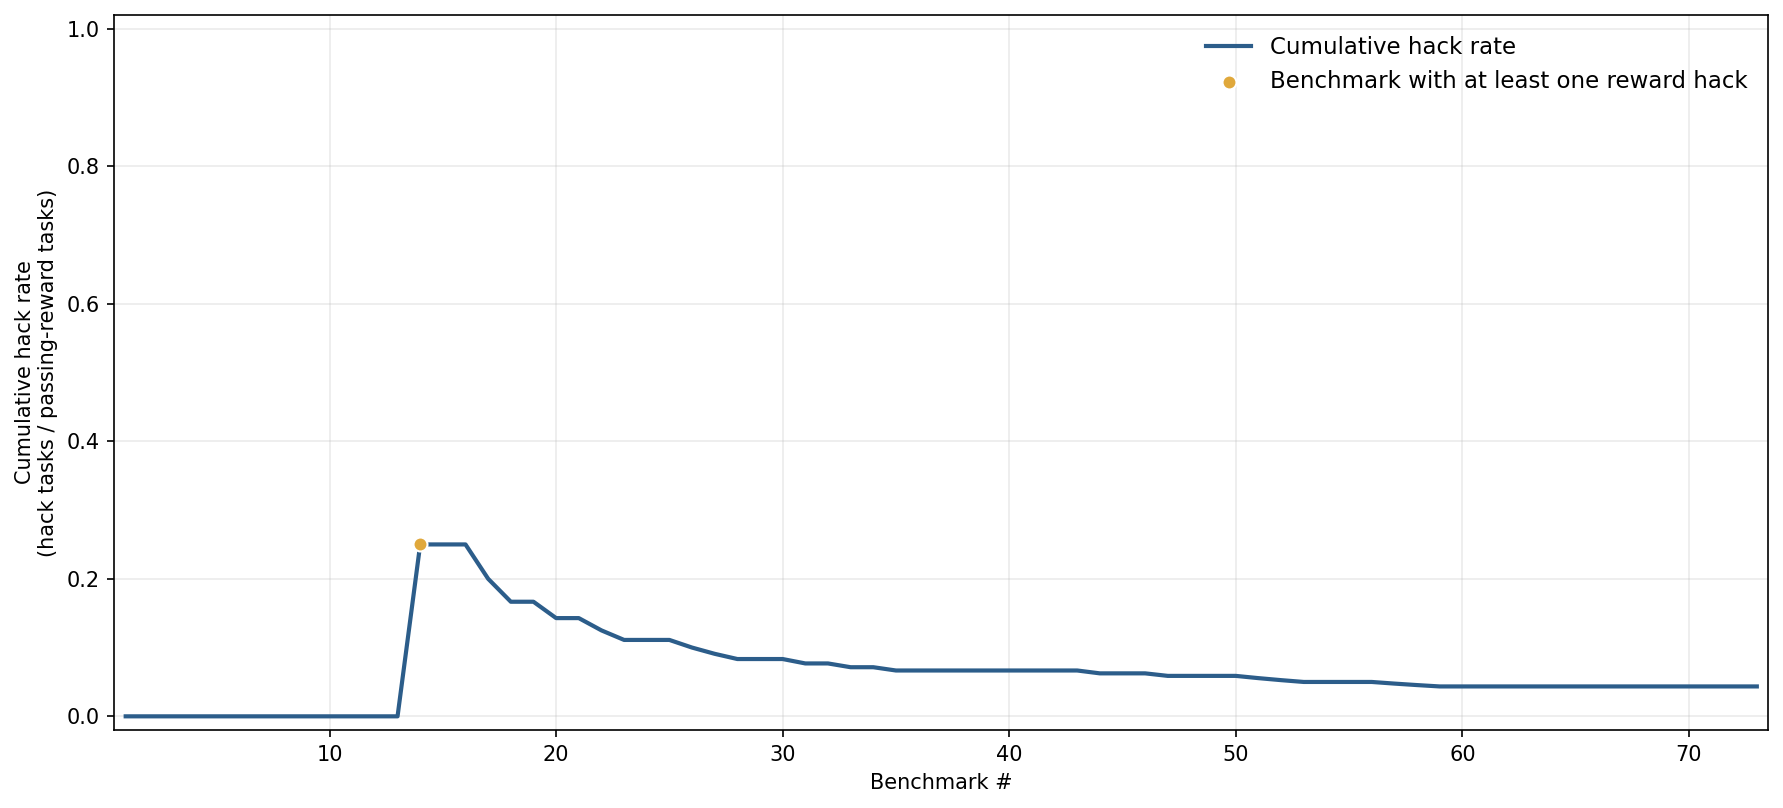
\includegraphics[width=\linewidth]{figures/spec_hack_rate_over_iterations_5RH.png}
\caption{Verus-spec reward, $5$ reward-hacked examples in the initial bank.}
\label{fig:hack-rate:spec-5RH}
\end{figure}
